\section{Task: Manage DB Schema}
\label{sec:task_manage_db_schema}

This task allows management of the database schema configuration and is reserved for expert users. It can not be run, but is performed using the GUI elements. \\

To make this task available use the 'Expert Mode' checkbox.

\begin{figure}[H]
  \hspace*{-2.5cm}
    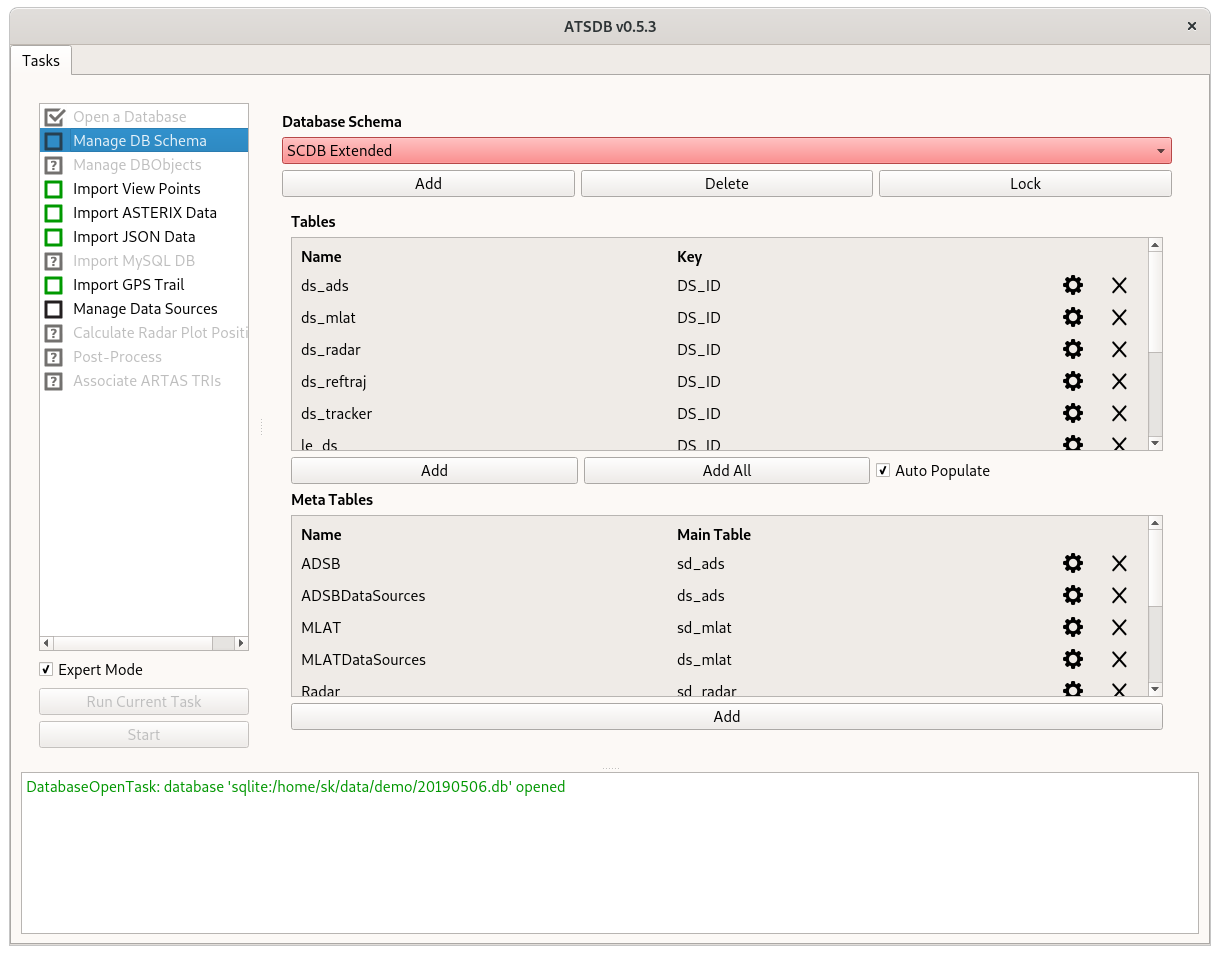
\includegraphics[width=19cm]{../screenshots/task_manage_schema.png}
  \caption{Task: Manage Schema}
\end{figure}

In this example, the current schema is shown in light red because it was not found in the empty database. As soon as data is imported, it is shown in a normal color. \\


\includegraphics[width=0.5cm]{../../data/icons/hint.png} For experienced users, a database schema can be created, edited and selected, which is currently not recommended (since it is not user friendly and might crash if used in the wrong manner).
